\textbf{Fernando\ Flores\ Labra}\\\\
\emph{Talca, 9 de enero de 1943}\\
Pol\'itico, fil\'osofo e ingeniero chileno, ex ministro de estado y actual senador de la Rep\'ublica.\\
Ingeniero comercial, doctor en filosof\'ia del lenguaje de la Universidad de Berkeley, fue ministro en dos
ocasiones del Presidente Salvador Allende y sufri\'o tres a\~nos de c\'arcel como preso pol\'itico durante
el r\'egimen de Augusto Pinochet por su participaci\'on en el gobierno de la Unidad Popular y su militancia Mapu.\\
Tras su liberaci\'on se instal\'o en California, Estados Unidos, donde desarroll\'o una intensa actividad acad\'emica
y empresarial.\\
Actualmente se desempe\~na como senador por la I Regi\'on de Tarapac\'a, por el período 2002-2010.\\
El 6 de noviembre de 2006, solicit\'o la suspensi\'on de su militancia del Partido por la Democracia (PPD), producto
de la -a su juicio- defensa que el partido le habr\'ia otorgado al senador Guido Girardi, tras el descubrimiento de la
entrega, por parte de \'este \'ultimo, de informaci\'on falsa al Servicio Electoral (Servel) respecto a sus gastos de
campa\~na en la \'ultima elecci\'on parlamentaria. El 9 de enero de 2007 present\'o su renuncia al partido.\\
En sus trabajos Flores plantea que gran parte de la coordinaci\'on humana ocurre en lo que denomin\'o "conversaciones
para la acci\'on", a trav\'es de las solicitudes, de las promesas y del cumplimiento de los compromisos entre las personas,
y sostuvo que la importancia de los computadores consiste en facilitar este trabajo de coordinaci\'on más que en el simple
procesamiento de datos.\\
Es fundador del Movimiento Atina Chile y Chile Primero (partido pol\'itico en formaci\'on) y corresponsal en diarios ciudadanos
como El Morrocotudo y El Rancahuaso.\\
Sus an\'alisis sobre las organizaciones humanas y el papel de la tecnolog\'ia desembocaron en diversos libros y en la creaci\'on
de empresas que desarrollaron software para la coordinaci\'on del trabajo en las organizaciones.\\
Entre sus obras destaca Understanding Computers and Cognition - A New Foundation for Design, publicado en 1986 junto a T. Winograd.\\
\begin{center}
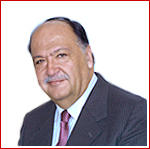
\includegraphics[height=3cm]{images/flores}
\end{center}
\begin{itemize}
	\item http://www.fernandoflores.cl
	\item http://www.chileprimero.cl
	\item http://www.atinachile.cl
\end{itemize}
